%%%%%%%%%%%%%%%%%%%%%%%%%%%%%%%%%%%%%%%%%%%%%%%%%%%%%%%%%%%%%%%%%%%%%%%%%%
% ------------------------------------------------------------------------
% LaTeX FHPaper Template by Thomas MIGLINCI
% ------------------------------------------------------------------------
%
% Das eigentliche Paper beginnt ab Zeile 124 - dort die Daten in den
% Aufruf von FHInfo eintragen.
%
% Bitte ersetzen Sie gegebenenfalls Master-Studiengang Mechatronik/Robotik durch Bachelor-.....
%
% Erstellt von T. Miglinci, Jänner 2012 und getestet von W. Kubinger, März 2012 und September 2012
%
% Letzte Änderung: 2.10.2015, WK	Neues Logo eingepflegt
%
%%%%%%%%%%%%%%%%%%%%%%%%%%%%%%%%%%%%%%%%%%%%%%%%%%%%%%%%%%%%%%%%%%%%%%%%%%

\documentclass[9pt,a4paper,twoside]{article}

\usepackage{graphicx}
\usepackage[utf8]{inputenc}
\usepackage[T1]{fontenc}
\usepackage[ngerman]{babel}%\datenaustrian

% mathematische Symbole
\usepackage{amsmath,amssymb,amsfonts,amstext}
%damit sind Bilder gezielter zu plazieren
\usepackage{float}

%%% ----------------------------------------------------------------------
\usepackage{color}
% Die Corporate Farben sind Blau (RGB 0/134/203), Grün (RGB 0/132/98) und Grau (RGB 98/107/113)
\definecolor{fhblue}{RGB}{0,134,203}
\newcommand\FHblue{\textcolor{fhblue}}
\definecolor{fhgruen}{RGB}{0,132,98}
\newcommand\FHgruen{\textcolor{fhgruen}}
\definecolor{fhgrau}{RGB}{98,107,113}
\newcommand\FHgrau{\textcolor{fhgrau}}

\unitlength1mm

% Zitierung im Harvard-Style
\usepackage{harvard}
\usepackage{url} %Darstellung von URLs erlauben
\citationstyle{dcu}  % für Zitate
\bibliographystyle{HarvardFHTWMR_V1_2e}% für Literaturverzeichnis
\citationmode{abbr}
\newcommand\citet{\citeasnoun}
\newcommand\citep{\cite}
% \citet(cootes01) -> Cootes (2001)
% \citep(cootes01) -> (Cootes, 2001)
\newcommand{\acessedthrough}{Available at:}%Für URL-Angabe
\newcommand{\acessedthroughp}{Available through:}%Für URL-Angabe (Geschützte Datenbank, Zugriff durch FH)
\newcommand{\acessedat}{Accessed}%Für URL-Datum-Angabe
\renewcommand{\harvardand}{\&}

% Seiten-Layout definieren
\usepackage[tmargin=14.5mm, bmargin=20mm, lmargin=20mm, rmargin=20mm,
            paper=a4paper,nofoot=true, nohead=true, noheadfoot=true]{geometry}

\usepackage{multicol}
\setlength{\columnsep}{7mm}

% weniger Warnungen wegen überfüllter Boxen
\tolerance = 9999
\sloppy

% Anpassung einiger Überschriften
\addto\captionsngerman
{
  \renewcommand\figurename{Abb.}
  \renewcommand\tablename{Tab.}
}

% Abbildungen, Gleichungen und Tabellen werden fortlaufend nummeriert
\renewcommand\thefigure{\arabic{figure}}
\renewcommand\thetable{\arabic{table}}
\renewcommand\theequation{\arabic{equation}}
\renewcommand\thesection{\arabic{section}.}
\renewcommand\thesubsection{\thesection\arabic{subsection}.}

\makeatletter
  % Überschriften neu definieren
  \renewcommand\section
  {
    \@startsection
    {section}{1}{0mm}      % für 'section', Ebene 1, 0mm Einzug
    {9pt} {6pt}            % Abstand darüber und darunter
    {\noindent\fontsize{10}{9pt}\scshape\textbf}%
  }

  \renewcommand\subsection
  {
    \@startsection
    {subsection}{2}{0mm}    % für 'subsection', Ebene 2, 0mm Einzug
    {9pt} {6pt}             % Abstand darüber und darunter
    {\noindent\fontsize{9}{9pt}\textbf}
  }
  \renewcommand\abstract[2]
  {
    \noindent\fontsize{9}{9pt}\textit{\textbf{Kurzfassung:} #1}\\
    \noindent\fontsize{9}{9pt}\textit{\textbf{Schlüsselwörter:} #2}
  }

  \newcommand\FHInfo[8]
  {
    \begin{multicols}{2}
      \fontsize{11}{14pt}
      \noindent{\textbf{\small Bachelor-Studiengang Mechatronik/Robotik}}\\
      {\fontsize{10}{20pt}
        \noindent \small FH Technikum Wien, Höchstädtplatz 6, A-1200 Wien\\
        \vspace{30pt}
      }
      \columnbreak
      \begin{figure}[H]
        \begin{flushright}
        \includegraphics[width=35mm,height=15mm,keepaspectratio=true]{#3}
        \label{fig:logo}
        \end{flushright}
      \end{figure}
    \end{multicols}
    \begin{center}
      \fontsize{12}{14pt}
      \noindent \textbf{\textsc {#4\\}}
      \bigskip
      {\fontsize{10}{12pt}
        \noindent{\textbf{Student: } #5, \textbf{PK: } #6}\\
        \noindent{\textbf{FH-BegutachterIn: } #7}\\
%        \noindent{\textbf{2.~BegutachterIn: } #8}
      }
    \end{center}
    \vspace{0mm}
  }
\makeatother


% --------------------------------------------------
% TITLE & AUTHOR
% --------------------------------------------------
\begin{document}

  \pagestyle{empty}  % keine Kopf- oder Fusszeile

  \FHInfo
    {Eintrag wird nicht verwendet}              % Eintrag wird nicht verwendet
    {Eintrag wird nicht verwendet}              % Eintrag wird nicht verwendet
    {./FHTW_Logo_Farbe_kr}                         % FH-Logo neu
    {Auslegung und Konstruktion eines Delta-Roboters zur Untersuchung der inversen Kinematik}                       % Titel der Arbeit
    {SCHAUSBERGER, Felix}                       % Student-Name
    {1610330049}                                % Student-PK-Nr
    {ABURAIA, Mohamed, MSc}                     % Name FH-Betreuer (1. BegutachterIn)
    {Titel NACHNAME, Vorname, Titel}            % Name Firmenbetreuer (2. BegutachterIn)

  \fontsize{9}{9pt}

  \begin{multicols}{2}
    \abstract
    {
        % Motivation
        % Stetig wachsender Einfluss technologiebezogener Industriebranchen machen den Erwerb technologischer Kompetenzen zu einem Schlüsselelement für den Erfolg künftiger Studentengenerationen. 
        Stetig zunehmende Relevanz der Automatisierung in diversen Industriebranchen machen den Erwerb technologischer Kompetenzen zu einem Schlüsselelement für den Erfolg künftiger Studentengenerationen.
        %
        % Problem - und Aufgabenstellung
        Trotz Bestrebungen von Bildungsreformen versucht ein Großteil des derzeitigen Lehrsystems weiterhin, Auszubildende auf die Zukunft vorzubereiten, indem Methoden der Vergangenheit angewandt werden. Aktuellen Bildungslehrplänen fehlt es häufig an Möglichkeiten, Studierenden Wechselwirkungen zwischen einzelnen Ingenieursgebieten zu vermitteln. Durch einen angemessenen Einstiegspunkt in die Konstruktion und Auslegung von Robotern könnte das vielseitige Feld angehenden Ingenieuren zugänglicher gemacht werden. 
        %
        % Methoden
        Diesbezüglich wird als Lösungsansatz in der vorliegenden Arbeit die mechatronische Auslegung und Konstruktion eines Robotersystems vorgestellt. Für diesen Zweck wird ein Prototyp einer parallelkinematischen Maschine, ein Delta-Roboter, entwickelt. Das System integriert anwendungsbezogen Wissen aus Mechanik, Elektrotechnik und Informatik. Um eine modulare Struktur zu ermöglichen wird der Aufbau mit ''smarten'' Antrieben realisiert. Infolgedessen kann der Roboter bei Anforderungsänderung dynamisch konfiguriert werden, um individuell auf spezielle Aufgaben angepasst zu werden. Die verwendeten Antriebe erleichtern, durch schnelles und kostengünstiges modulieren, die Entwicklung. Darüber hinaus wird, in Kombination mit Open-Source-Software, kein spezielles industrielles Equipment benötigt. 
        %
        % Zusammenfassung und Ergebnisse
        Die Ergebnisse zeigen, dass durch die genannten Vorteile ein Prototyp für didaktische Zwecke in der akademischen Ausbildung eigensicher, transportabel und kostengünstig hergestellt werden kann.
    } {Delta-Roboter, Parallelroboter, Modellierung von Robotern, Rekonfigurierbarer Roboter}

    \section{Einleitung}
        
        \noindent
        %%%%%%%%%%%%%%%%%%%%%%%%%%%%%%%%%%%%%%%%%%%%%%%%%%%%
        %%                 SMART ENGINES                  %%
        %%%%%%%%%%%%%%%%%%%%%%%%%%%%%%%%%%%%%%%%%%%%%%%%%%%%
        Robotik und Automatisierung revolutionieren zusammen mit ''Smart Manufacturing'' gegenwärtig nahezu die gesamte moderne Fertigungsindustrie \cite{FrDe18,TaQi19}. Die erschlossenen Technologien stellen in vielen Bereichen, darunter der automatisierten Fertigung, der Medizin und dem Gesundheitswesen, der Altenpflege und Rehabilitation, der unbemannten Suche und Rettung sowie der Automobilindustrie bereits etablierte Systeme dar \cite{Eg14,SaDa18}. 
        % Schon mit derzeitigen Verfahrensweisen sind Roboter in der Lage, zahlreiche Aufgaben effizienter und konsistenter als konventionelle Fertigungsprozesse mit menschlicher Belegschaft zu erledigen \cite{FrDe18}.
        ''Smart Manufacturing'' erfordert die Interaktion, Integration und Fusion physischer und informatischer, softwaretechnischer Komponenten. In Anbetracht dessen verfolgen aktuelle Trendkonzepte das gemeinsame Ziel einer ''Smart Factory'', in der cyber-physische Systeme die physischen Prozesse der Fabrik überwachen und dezentrale Entscheidungen treffen. Im Zuge dessen gewinnen ''smarte'' Antriebe mit kontinuierlicher Überwachung des eigenen Zustands, Kommunikation untereinander, dezentraler Datenverarbeitung über Edge-Computing und dem Übertragen von Nutzdaten und relevanten Informationen in eine Cloud immer mehr an Bedeutung.\\
        \\
        %%%%%%%%%%%%%%%%%%%%%%%%%%%%%%%%%%%%%%%%%%%%%%%%%%%%
        %%                     HEBI                       %%
        %%%%%%%%%%%%%%%%%%%%%%%%%%%%%%%%%%%%%%%%%%%%%%%%%%%%
        Die verwendeten Modelle der kommerziell erwerbbaren, modularen Roboterantriebe HEBI X5-1 verfolgen dieses Konzept der ''smarten'' Aktoren. Obwohl die derzeit im konventionellen Handel erhältlichen Robotersysteme bereits in der Lage sind, einen Großteil des Anwendungsgebietes für Manipulatoren abzudecken, erweitert die dynamisch konfigurierbare Struktur der HEBI Antriebe diesen Bereich um die Möglichkeit, das System individuell auf spezielle Aufgaben anzupassen. Die spezielle Bauweise ermöglicht Roboterstrukturen skalierbarer Komplexität kostengünstig zu entwickeln und fördert das gesamte Gebiet der Ingenieurswissenschaften, indem anwendungsbezogen Wissen aus Mechanik, Elektrotechnik und Informatik in einem geschlossenen System integriert wird.

    \section{Problem- und Aufgabenstellung}
        
        \noindent
        Die vorliegende Arbeit beschäftigt sich mit der mechatronischen Auslegung eines parallelkinematischen Delta-Roboters, um Studierenden die Möglichkeit zu bieten, anwendungsbezogen Kompetenzen im interdisziplinären Gebiet der Ingenieurswissenschaften zu erwerben. Denn obgleich sich die heutige, schnelllebige Welt und ihre Wirtschaftssysteme rasant verändern, hat die öffentliche Bildung seit ihrer Einführung nahezu dasselbe System beibehalten. Allerdings ist durch den stetig wachsenden Einfluss technologiebezogener Branchen der Erwerb technologischer Kompetenzen durch die Integration von Ingenieurwissenschaften in den Lehrplan ein Schlüsselelement für den Erfolg künftiger Studentengenerationen \cite{Eg14}. Um einen für didaktische Zwecke geeigneten Roboter zu entwerfen, ist
        im Betriebszustand die Sicherheit für Mensch und Maschine zu gewährleisten, während aufgrund wechselnder Räumlichkeiten der Aufbau portabel gestaltet werden muss. Daraus resultieren Anforderungen einer möglichst kompakten als auch eigensicheren, robusten aber dennoch kostengünstigen Konstruktion.

    \section{Materialien und Methoden}
        
        \noindent
        Die Arbeit beschäftigt sich anfangs mit der geometrischen und mathematischen Modellierung des Systems. Die Vorgehensweise hierfür war zunächst die Bestimmung der Freiheitsgrade sowie die Berechnung des Modells der inversen Kinematik des Delta-Roboters. Nach erfolgreichem Abschluss der Konzeptionsphase wurde anschließend ein Prototyp konstruiert und programmiert, um das entworfene Modell am Testaufbau auf Richtigkeit überprüfen zu können. Als Fertigungsverfahren wurde hierbei Rapid Prototyping eingesetzt. Die Steuerungsarchitektur wurde in MathWorks\textregistered\ MATLAB (von engl. MATrix LABoraty) mithilfe der von HEBI zur Verfügung gestellten Programmierschnittstelle numerisch implementiert.
        % Systemtests und Konfigurationen der Module wurden in Scope, einer von HEBI angebotenen GUI zur Überwachung der Motoren und zum Senden manueller Befehlen, durchgeführt.
        Den Abschluss der Arbeit bildet die \textit{Jacobi-Matrix}, welche den Zusammenhang zwischen den Gelenkgeschwindigkeiten und der Geschwindigkeit des Endeffektors im kartesischen Raum beschreibt und als Grundlage für weiterführende Arbeiten dient.

    \section{Praktische Durchführung}
        
        \noindent
        Die Verbindungsstücke zwischen den einzelnen Gliedern sind in der CAD-Software (von engl. Computer-Aided Design) SolidWorks konstruiert und mit der additiven Fertigungsmethode des selektiven Lasersinterns gefertigt. 
        % (SLS) in einem eos P100 SLS Drucker
        Abbildung \ref{fig:delta-attached-isometric-view} zeigt den kompletten Aufbau des in SolidWorks entworfenen Robotersystems. 
        \begin{figure}[H]%
            \fbox{%
                \begin{minipage}{8.1cm}%
                    \begin{center}%
                        % 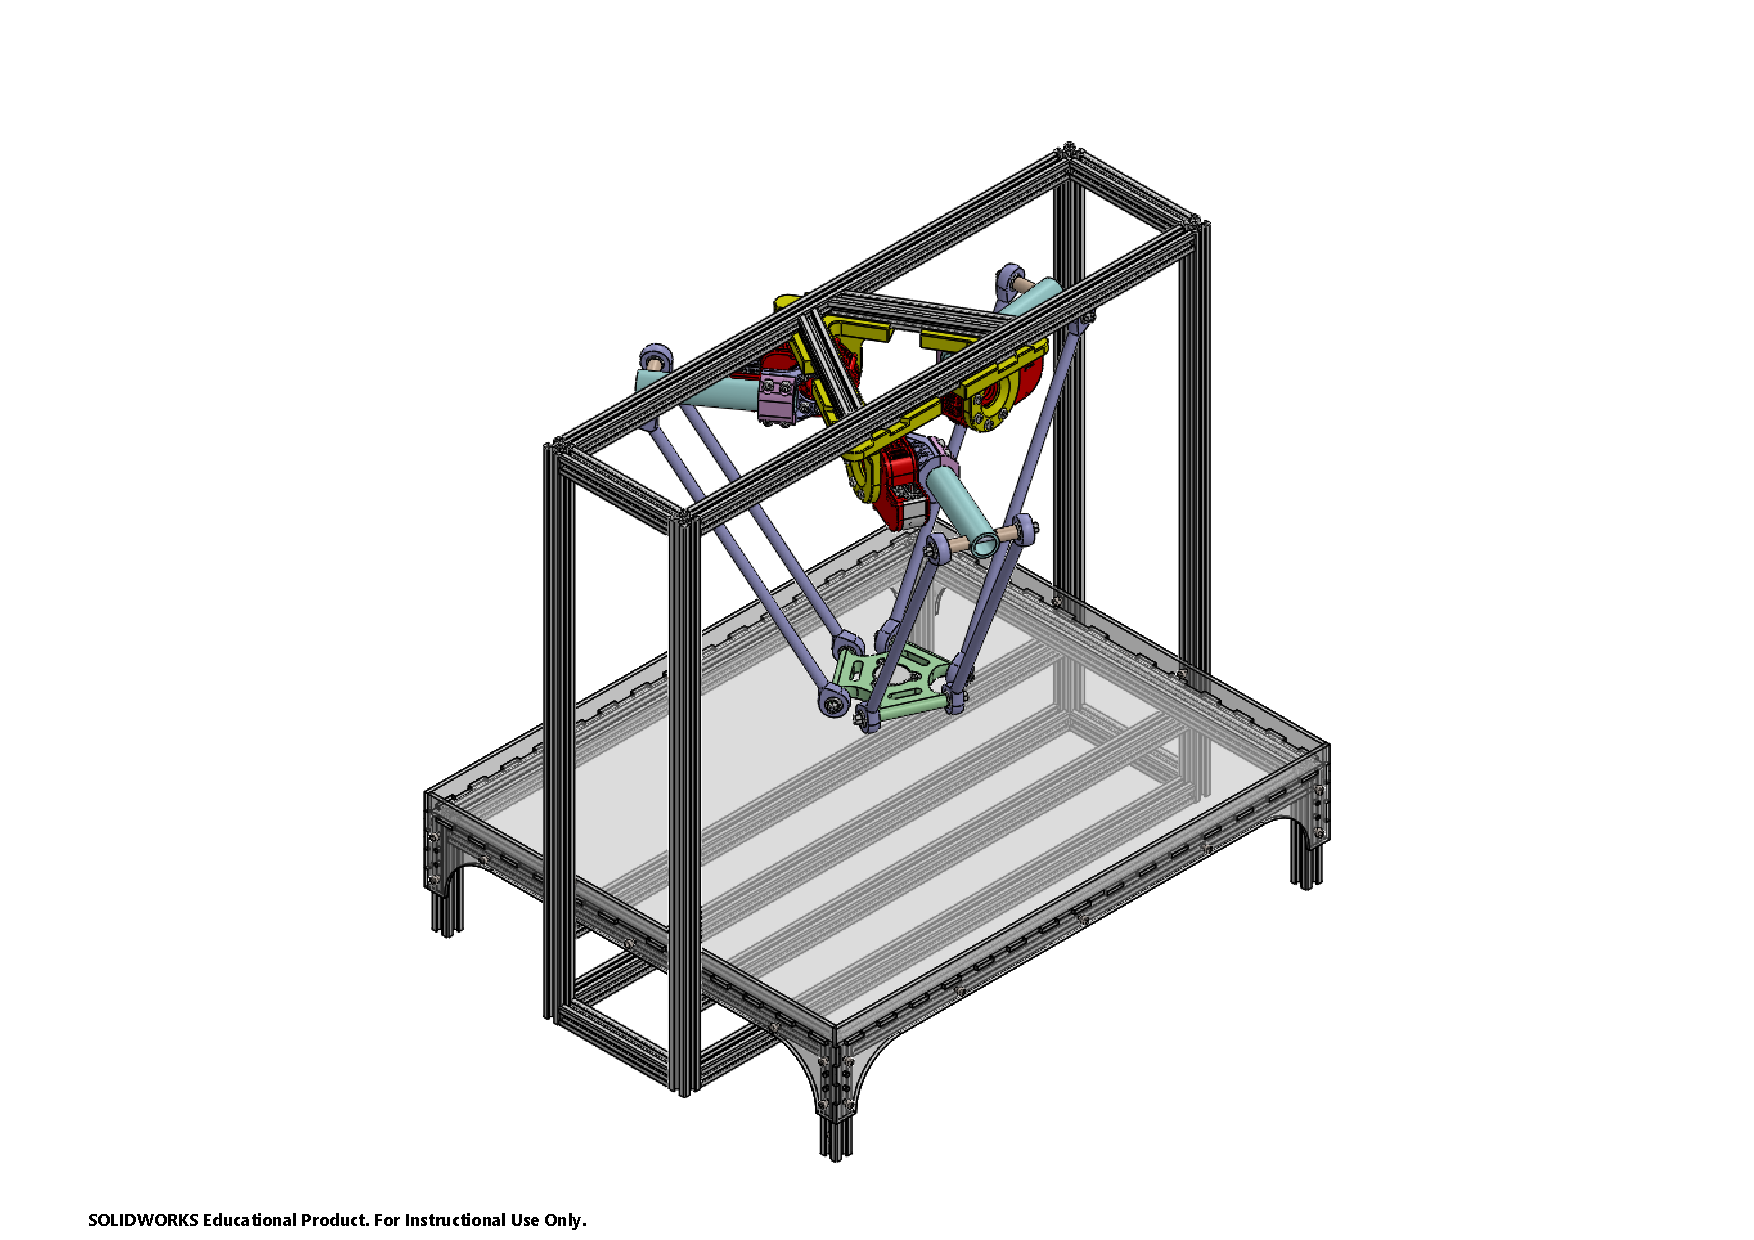
\includegraphics[width=80mm]{./delta-attached-isometric-view}%
                        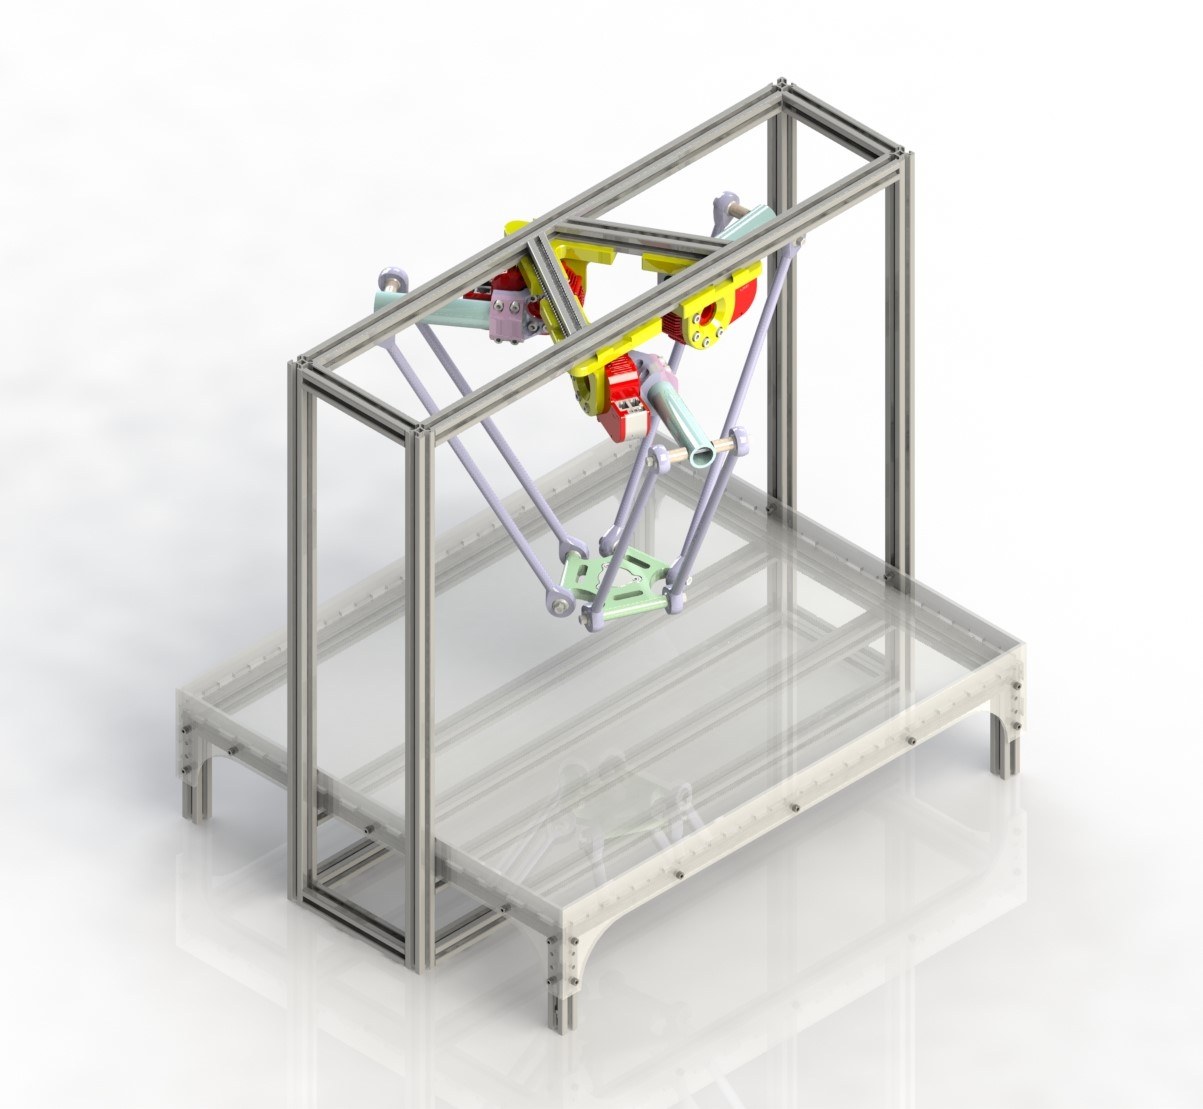
\includegraphics[width=80mm]{./delta-attached-isometric-view-rendered-1}%
                    \end{center}%
                \end{minipage}%
            }%
            \caption[Isometrische Ansicht des Delta-Roboters]{Isometrische Ansicht des Delta-Roboters}%
            \label{fig:delta-attached-isometric-view}%
        \end{figure}%
        \noindent
        Die proximalen Glieder sind über robolink\textregistered\ W Aluminiumrohre und die distalen  über igubal\textregistered-Doppelgelenklager KDGM der Firma IGUS realisiert. Der Rahmen und Arbeitsbereich des Roboters sind aus 20 $[mm]$ Aluminiumprofilen und die Ebenen aus 4 $[mm]$ starken Plexiglasplatten gefertigt. Bei der Baugröße und den Befestigungsmöglichkeiten wurde darauf geachtet, den Roboter benutzerfreundlich, kompakt und modular zu gestalten, um Erweiterungen zu ermöglichen und Wartungsarbeiten zu erleichtern.

    \section{Ergebnisse}
        
        \noindent
        Die Ergebnisse zeigen, dass ein Prototyp für didaktische Zwecke eigensicher, transportabel und kostengünstig hergestellt werden kann um angehenden Ingenieuren die einzigartige Möglichkeit zu bieten, parallelkinematische Maschinen praxisorientiert zu studieren. Die vorliegende Arbeit hat das gewünschte Ziel, die mechatronische Auslegung eines Delta-Roboters für den Einsatz in der akademischen Ausbildung zu entwickeln, erfüllt. Der Aufbau bestätigt die Funktionsfähigkeit der Algorithmen und zeigt, dass das System wie erwartet bei bekannter Pose des Endeffektors die entsprechenden Gelenkwinkel liefert und der Steuerung zur Trajektorienplanung übergibt.

    \section{Zusammenfassung und Ausblick}
    
        \noindent
        In der vorliegenden Arbeit wird die mechatronische Auslegung eines Delta-Roboters für den Einsatz in der akademischen Ausbildung vorgestellt.
        % Eine Herausforderung in der Entwicklung paralleler Robotersysteme liegt in der mathematischen Modellierung sowie in der Auslegung der Mechanik der simultan ablaufenden, räumlichen Bewegungen des Roboters. 
        Um einen für Ausbildungszwecke geeigneten Roboter zu konstruieren, muss im Betriebszustand die Sicherheit für Mensch und Maschine gewährleistet werden, während aufgrund wechselnder Räumlichkeiten der Aufbau portabel gestaltet sein muss. Daraus resultieren Anforderungen einer möglichst eigensicheren, robusten aber dennoch kostengünstigen Konstruktion.\\
        \\
        In weiterführenden Arbeiten kann die verwendete Regelungsstrategie optimiert werden, um das dynamische Verhalten des Roboters zu verbessern. Um die Positionier- und Wiederholgenauigkeit zu verfeinern kann einerseits eine angemessene Trajektorienplanung ausgelegt werden, andererseits können zu diesem Zweck auch die Fertigungs- und Montagetoleranzen der mechanischen Struktur optimiert werden. Zu dem können auch die Algorithmen verbessert werden, indem diese zum Beispiel zeitoptimiert werden. Darüber hinaus können die Parameter zur Linearisierung der Pfade optimiert werden.  Abschließend können sich zukünftige Arbeiten mit Arbeitsraumanalysen,
        Singularitätsuntersuchungen sowie dynamischen Modellierungen des Roboters befassen.
    
    \section{Literaturverzeichnis}
    {
      \renewcommand{\refname}{\vspace{-5mm}} % keine eigene Überschrift durch \bibliography...
      \linespread{.8}\selectfont
      \bibliography{Literatur}
    }

  \end{multicols}

\end{document}
